% =====================================================================
%  V2V-Project -- Study Pack
%  Section S9 : Security Evaluation
%  Source file studied: tests/evaluate_security.py
%  Standalone document -- compile with:  pdflatex 09-security-evaluation.tex
% =====================================================================
\documentclass[11pt,a4paper]{article}

\usepackage[utf8]{inputenc}
\usepackage[T1]{fontenc}
\usepackage{lmodern}

\usepackage[a4paper,margin=2.4cm]{geometry}
\usepackage{enumitem}
\setlist{topsep=2pt,itemsep=2pt}

\usepackage{amsmath}
\usepackage{amssymb}
\usepackage{booktabs}
\usepackage{graphicx}
\usepackage{xcolor}
\usepackage{listings}
\usepackage{tikz}
\usetikzlibrary{arrows.meta,positioning,shapes.geometric,calc,fit,backgrounds}
\usepackage[colorlinks=true,linkcolor=blue,urlcolor=blue,citecolor=blue]{hyperref}

\definecolor{codebg}{rgb}{0.97,0.97,0.94}
\definecolor{codegreen}{rgb}{0.00,0.50,0.00}
\definecolor{codegray}{rgb}{0.50,0.50,0.50}
\definecolor{keyblue}{rgb}{0.00,0.20,0.70}
\definecolor{boxblue}{rgb}{0.88,0.93,1.00}
\definecolor{boxyellow}{rgb}{1.00,0.97,0.85}

\lstdefinestyle{py}{
  language=Python,
  backgroundcolor=\color{codebg},
  basicstyle=\ttfamily\footnotesize,
  keywordstyle=\color{keyblue}\bfseries,
  stringstyle=\color{codegreen},
  commentstyle=\color{codegray}\itshape,
  numberstyle=\tiny\color{codegray},
  numbers=left,
  numbersep=8pt,
  showstringspaces=false,
  breaklines=true,
  breakatwhitespace=false,
  frame=single,
  rulecolor=\color{codegray},
  tabsize=4,
  captionpos=b,
}
\lstdefinestyle{term}{
  backgroundcolor=\color{codebg},
  basicstyle=\ttfamily\footnotesize,
  breaklines=true,
  frame=single,
  rulecolor=\color{codegray},
  numbers=none,
  captionpos=b,
}

\title{\textbf{V2V-Project Study Pack}\\[4pt]
       \large Section S9 --- Security Evaluation}
\author{Information Security Project --- Beginner Study Notes}
\date{Source file: \texttt{tests/evaluate\_security.py}}

\begin{document}
\maketitle
\tableofcontents
\newpage

% =====================================================================
\section{Title and ``What You'll Learn''}
% =====================================================================

\subsection*{Section Title}
\textbf{S9 --- Security Evaluation: a script that \emph{measures} the project ---
how fast the cryptography runs and how reliably the defences catch attacks ---
and prints a pass/fail report.}

\subsection*{Plain-English Summary (read this first)}
Section~S8 \emph{proved} the defences work by attacking them once each. Section~S9
goes further: it \emph{measures} them, many times over, and writes the numbers
down. One script, \texttt{evaluate\_security.py}, runs six tests. Three are
\textbf{speed} tests --- can the encryption, decryption and signing keep up with
a car sending messages in real time? Three are \textbf{correctness} tests --- do
the replay and tamper defences catch \emph{100\%} of attacks, and are the random
nonces truly unique? Every test has a numeric \textbf{target}; the script prints
a table of \texttt{PASS} / \texttt{FAIL} and saves it to a report file. S9 is the
\emph{evidence} behind the project's security claims.

\subsection*{Learning Outcomes}
After studying this section you will be able to:
\begin{itemize}
  \item Explain \textbf{benchmarking} and what \textbf{throughput} (ops/second) means.
  \item Explain why a \textbf{high-resolution timer} is used for measurement.
  \item Explain a \textbf{detection rate} and why 100\% is the target.
  \item Explain \textbf{nonce uniqueness} and, briefly, the \emph{birthday problem}.
  \item Walk through all six test functions and the report formatter.
  \item Run the evaluation, read the table, and explain every row.
  \item Explain the difference between \emph{measuring} and \emph{proving} security.
\end{itemize}

% =====================================================================
\section{Where This Fits}
% =====================================================================

S9 sits \emph{above} the whole pipeline as its report card. The earlier sections
\emph{build} the defences and S8 \emph{attacks} them once; S9 \emph{quantifies}
them. It imports the real crypto functions (S3) and the real
\texttt{ReplayCache} (S4) and runs them thousands of times to produce hard
numbers --- both for \emph{performance justification} (``ECDSA and AES are fast
enough for V2V'') and for \emph{security evidence} (``replay and tamper detection
are 100\%'').

\begin{center}
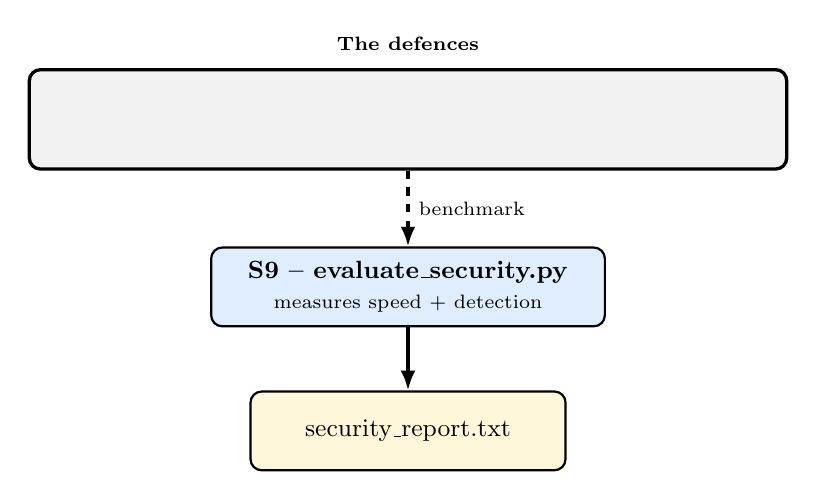
\begin{tikzpicture}[font=\small,node distance=7mm and 9mm,
   st/.style={draw,rounded corners,minimum width=2.5cm,minimum height=1.0cm,
              align=center,thick}]
  \node[st,fill=red!12]   (cr) {Crypto\\\scriptsize S3};
  \node[st,fill=green!12,right=of cr] (au) {Handshake\\\scriptsize S4};
  \node[st,fill=boxyellow,right=of au] (ms) {Messaging\\\scriptsize S5};
  \node[draw,very thick,rounded corners,fill=gray!10,fit=(cr)(au)(ms)] (sys) {};
  \node[above=1mm of sys,font=\scriptsize\bfseries] {The defences};
  \node[st,fill=boxblue,below=11mm of au,minimum width=5cm] (ev)
       {\textbf{S9 -- evaluate\_security.py}\\\scriptsize measures speed + detection};
  \draw[-{Latex[length=2.5mm]},very thick,dashed] (sys) -- (ev)
       node[midway,right,font=\scriptsize]{benchmark};
  \node[st,fill=boxyellow,below=8mm of ev,minimum width=4cm] (rep) {security\_report.txt};
  \draw[-{Latex[length=2.5mm]},very thick] (ev) -- (rep);
\end{tikzpicture}
\end{center}

% =====================================================================
\section{The Theory You Must Study}
% =====================================================================

\subsection{Benchmarking and Throughput}
\textbf{Plain definition.} \emph{Benchmarking} means measuring how fast a piece
of code runs, under controlled, repeatable conditions. \emph{Throughput} is the
amount of work done per unit time --- here, \textbf{operations per second}
(ops/s).

\textbf{Real-life analogy.} Timing how many envelopes a person can seal in one
minute. Do it once and it is a fluke; do it over a thousand envelopes and you
have a trustworthy rate.

\textbf{Why it exists.} A real car sends safety messages many times a second. If
encrypting or signing one message were slow, the security would make the car
\emph{unsafe} by lagging. Benchmarking answers: ``is the cryptography fast enough
for real time?''

\textbf{How it works here.} Each speed test runs an operation in a loop many
times (1000 for encryption/decryption, 100 for signing), measures the total time,
and computes \texttt{ops = iterations / elapsed}.

\textbf{Security property it relates to.} Indirectly all of them --- it shows the
defences are \emph{practical}, not just correct.

\subsection{High-Resolution Timing (\texttt{time.perf\_counter})}
\textbf{Plain definition.} \texttt{time.perf\_counter()} is a clock designed for
measuring short \emph{durations} very precisely.

\textbf{Real-life analogy.} A stopwatch, not a wall clock. A wall clock tells you
the time of day; a stopwatch is built to measure how long something \emph{took}.

\textbf{Why it exists.} An ordinary clock can jump (e.g.\ when the operating
system adjusts the time) and is too coarse for sub-millisecond work.
\texttt{perf\_counter} is steady and fine-grained, so a benchmark is accurate.

\textbf{How it works here.} The pattern is: \texttt{start = time.perf\_counter()},
run the loop, then \texttt{elapsed = time.perf\_counter() - start}.

\textbf{Security property it relates to.} None directly --- it makes the
measurement trustworthy.

\subsection{Pass/Fail Thresholds}
\textbf{Plain definition.} A \emph{threshold} is a fixed target a measurement
must beat to count as a pass.

\textbf{Real-life analogy.} A driving test: parallel-park within a set time or you
fail. The number is decided in advance, so the result is objective.

\textbf{Why it exists.} ``Fast'' and ``reliable'' are vague. A threshold turns a
measurement into a clear yes/no, and makes the report honest --- you cannot move
the goalposts after seeing the result.

\textbf{How it works here.} Encryption and decryption must exceed
\textbf{500 ops/s}; signing must exceed \textbf{100 ops/s}; detection tests must
be \textbf{100\%}; nonce collisions must be \textbf{0}. Each test sets
\texttt{passed = (measurement\ meets\ target)}.

\textbf{Security property it relates to.} It makes every other property
\emph{measurable} rather than asserted.

\subsection{Detection Rate}
\textbf{Plain definition.} A \emph{detection rate} is the fraction of attacks a
defence catches: \emph{caught divided by total}.

\textbf{Real-life analogy.} A metal detector at an airport: if 100 weapons go
through and it catches 100, the detection rate is 100\%. Catching 99 is not good
enough.

\textbf{Why it exists.} Catching an attack ``usually'' is a false comfort --- a
single missed tampered message could cause a crash. The only acceptable target
for these defences is \textbf{100\%}.

\textbf{How it works here.} \texttt{test\_replay\_detection} adds 100 nonces to a
\texttt{ReplayCache}, then re-adds each and counts how many raise
\texttt{ReplayError}; it must be 100/100. \texttt{test\_tamper\_detection}
encrypts 50 messages, flips a byte in each, and counts how many decryptions
raise \texttt{DecryptionError}; it must be 50/50.

\textbf{Security property it relates to.} \textbf{Replay prevention} and
\textbf{integrity}.

\subsection{Nonce Uniqueness and the Birthday Problem}
\textbf{Plain definition.} A \emph{nonce} must never repeat. \emph{Nonce
uniqueness} testing checks that a batch of randomly generated nonces contains no
duplicates (\emph{collisions}). The \emph{birthday problem} is the surprising
fact that collisions become likely much sooner than intuition suggests --- but
only when the pool of possible values is small.

\textbf{Real-life analogy.} In a room of just 23 people, two probably share a
birthday --- because there are only 365 possible days. But if ``birthdays'' could
be any of $2^{256}$ values, you would need an unimaginable crowd before a clash.

\textbf{Why it exists.} If two messages reused a nonce, AES-GCM's security would
break. The test gives empirical confidence that \texttt{os.urandom} is producing
fresh values.

\textbf{How it works here.} \texttt{test\_nonce\_uniqueness} generates 10{,}000
nonces of 32 bytes (256 bits) each, puts them in a \texttt{set} (which discards
duplicates), and checks \texttt{collisions = count - len(set)} is 0. With 256-bit
values, 10{,}000 draws colliding is so unlikely it is effectively impossible ---
so a result of 0 is expected every run.

\textbf{Security property it relates to.} It underpins \textbf{confidentiality}
(AES-GCM relies on unique nonces).

\subsection{Measuring vs Proving Security}
\textbf{An important distinction.} S9 \emph{measures}; it does not mathematically
\emph{prove}. A 100\% detection rate over 100 trials is strong \emph{evidence},
but it is not a proof that the defence can \emph{never} fail. Real security
assurance combines testing (like S9), code review, and reasoning about the
underlying mathematics. Being clear about this is part of doing evaluation
honestly --- the script produces a \emph{report}, not a \emph{theorem}.

% =====================================================================
\section{Code Walkthrough}
% =====================================================================

\texttt{evaluate\_security.py} has a header helper, six test functions, a table
formatter, and a \texttt{main} that runs everything and saves a report.

\subsection{The three speed tests}
\begin{lstlisting}[style=py,caption={evaluate\_security.py --- a representative speed benchmark.}]
def test_encryption_speed(iterations: int = 1000) -> dict:
    """Benchmark AES-256-GCM encryption throughput."""
    key = os.urandom(32)
    payload = b"test BSM payload " * 10           # ~170 bytes (realistic BSM)

    start = time.perf_counter()
    for _ in range(iterations):
        aes_gcm_encrypt(key, payload)
    elapsed = time.perf_counter() - start

    ops = iterations / elapsed
    passed = ops > 500
    return {"name": "Encryption Speed", "result": f"{ops:.0f} ops/s",
            "target": ">500", "passed": passed}
\end{lstlisting}
\textbf{Step by step:}
\begin{enumerate}
  \item Make a 32-byte AES key and a ~170-byte payload (about the size of a real
        BSM).
  \item Read the high-resolution clock into \texttt{start}.
  \item Run \texttt{aes\_gcm\_encrypt} 1000 times in a loop.
  \item Read the clock again; \texttt{elapsed} is the total time.
  \item \texttt{ops = iterations / elapsed} is the throughput in operations per
        second.
  \item \texttt{passed} is \texttt{True} if \texttt{ops} beats the 500 ops/s
        threshold.
  \item Return a small dictionary with the name, result, target and pass flag.
\end{enumerate}
\texttt{test\_decryption\_speed} is identical but times \texttt{aes\_gcm\_decrypt}
(it encrypts once first to get something to decrypt). \texttt{test\_signature\_speed}
times \texttt{ecdsa\_sign} over 100 iterations with a target of 100 ops/s ---
signing is slower than symmetric encryption, so it has a lower bar.
\textbf{Theory link:} benchmarking; throughput; \texttt{perf\_counter};
thresholds.

\subsection{test\_replay\_detection() --- 100\% replay catching}
\begin{lstlisting}[style=py,caption={evaluate\_security.py --- the replay detection test.}]
def test_replay_detection(count: int = 100) -> dict:
    cache = ReplayCache(window_seconds=300)
    nonces = [os.urandom(32).hex() for _ in range(count)]
    for n in nonces:
        cache.check_and_add(n)              # first time: accepted

    caught = 0
    for n in nonces:
        try:
            cache.check_and_add(n)          # second time: must be rejected
        except ReplayError:
            caught += 1

    passed = caught == count
    return {"name": "Replay Detection Rate", "result": f"{caught}/{count}",
            "target": "100%", "passed": passed}
\end{lstlisting}
\textbf{Step by step:}
\begin{enumerate}
  \item Create a \texttt{ReplayCache} and generate 100 unique random nonces.
  \item Add each nonce once --- all are new, so all are accepted.
  \item Try to add every nonce a \emph{second} time. Each repeat \emph{must}
        raise \texttt{ReplayError}; \texttt{caught} counts how many do.
  \item The test passes only if \texttt{caught == 100} --- a 100\% detection rate.
\end{enumerate}
\textbf{Theory link:} detection rate; the \texttt{ReplayCache} of S4. This is the
quantified version of the S8 replay attack --- not one replay, but 100.

\subsection{test\_tamper\_detection() --- 100\% tamper catching}
\begin{lstlisting}[style=py,caption={evaluate\_security.py --- the tamper detection test.}]
def test_tamper_detection(count: int = 50) -> dict:
    key = os.urandom(32)
    caught = 0
    for _ in range(count):
        ct, nonce, tag = aes_gcm_encrypt(key, b"test BSM payload " * 10)
        tampered = bytearray(ct)
        if tampered:
            tampered[len(tampered) // 2] ^= 0x01      # flip one bit
        try:
            aes_gcm_decrypt(key, bytes(tampered), nonce, tag)
        except DecryptionError:
            caught += 1
    passed = caught == count
    return {"name": "Tamper Detection Rate", "result": f"{caught}/{count}",
            "target": "100%", "passed": passed}
\end{lstlisting}
\textbf{Step by step:}
\begin{enumerate}
  \item For each of 50 rounds: encrypt a payload, then flip \emph{one bit}
        (\texttt{\^{}= 0x01}) in the middle of the ciphertext.
  \item Try to decrypt the tampered ciphertext. AES-GCM's tag will not match, so
        \texttt{aes\_gcm\_decrypt} raises \texttt{DecryptionError};
        \texttt{caught} is incremented.
  \item The test passes only if all 50 tampered messages were caught --- 50/50.
\end{enumerate}
\textbf{Theory link:} detection rate; AES-GCM integrity (S3). Note it flips just
\emph{one bit} --- the smallest possible change --- and even that is always
caught.

\subsection{test\_nonce\_uniqueness() --- no collisions}
\begin{lstlisting}[style=py,caption={evaluate\_security.py --- the nonce uniqueness test.}]
def test_nonce_uniqueness(count: int = 10000) -> dict:
    nonces = set()
    for _ in range(count):
        nonces.add(os.urandom(32).hex())
    collisions = count - len(nonces)
    passed = collisions == 0
    return {"name": f"Nonce Uniqueness ({count//1000}k)",
            "result": f"{collisions} collisions", "target": "0", "passed": passed}
\end{lstlisting}
\textbf{Step by step:}
\begin{enumerate}
  \item Generate 10{,}000 random 32-byte nonces, adding each to a \texttt{set}.
  \item A \texttt{set} automatically discards duplicates, so if any nonce
        repeated, \texttt{len(nonces)} would be less than \texttt{count}.
  \item \texttt{collisions = count - len(nonces)} --- expected to be 0.
  \item The test passes if there were zero collisions.
\end{enumerate}
\textbf{Theory link:} nonce uniqueness; the birthday problem. With 256-bit
nonces, 10{,}000 draws colliding is astronomically unlikely.

\subsection{format\_table() and main()}
\texttt{format\_table} takes the list of result dictionaries and draws a neat
ASCII table with columns \emph{Test}, \emph{Result}, \emph{Target},
\emph{Status}, then an ``Overall: X/Y tests PASSED'' line. \texttt{main} calls
all six test functions, prints the table, and writes it (with a timestamp) to
\texttt{tests/security\_report.txt} so there is a saved record.

% =====================================================================
\section{Hands-On / Practical}
% =====================================================================

\subsection{Run the evaluation}
\begin{lstlisting}[style=term]
python tests\evaluate_security.py
\end{lstlisting}

\noindent\textbf{Expected output (sample --- speed numbers vary by computer):}
\begin{lstlisting}[style=term]
========================================================
     V2V SECURITY EVALUATION REPORT
========================================================

+-----------------------------+----------------+----------+----------+
| Test                        | Result         | Target   | Status   |
+=============================+================+==========+==========+
| Encryption Speed            | 121840 ops/s   | >500     | PASS     |
| Decryption Speed            | 118905 ops/s   | >500     | PASS     |
| Signature Speed             | 6730 ops/s     | >100     | PASS     |
| Replay Detection Rate       | 100/100        | 100%     | PASS     |
| Tamper Detection Rate       | 50/50          | 100%     | PASS     |
| Nonce Uniqueness (10k)      | 0 collisions   | 0        | PASS     |
+-----------------------------+----------------+----------+----------+

Overall: 6/6 tests PASSED

Report saved to: tests/security_report.txt
\end{lstlisting}

\subsection{What each row means}
\begin{itemize}
  \item \textbf{Encryption / Decryption Speed} --- tens of thousands of
        operations per second, far above the 500 needed; AES-256-GCM is
        comfortably fast enough for a car sending one BSM per second.
  \item \textbf{Signature Speed} --- a few thousand signings per second; ECDSA is
        slower than symmetric encryption (it is public-key maths) but still well
        past its 100 ops/s bar.
  \item \textbf{Replay Detection Rate 100/100} --- every one of 100 repeated
        nonces was caught by the \texttt{ReplayCache}.
  \item \textbf{Tamper Detection Rate 50/50} --- every one-bit change in 50
        messages was caught by AES-GCM.
  \item \textbf{Nonce Uniqueness 0 collisions} --- 10{,}000 random nonces, all
        distinct.
  \item \textbf{Overall 6/6} --- every test met its target.
\end{itemize}

\subsection{Try This Yourself (mini-experiment)}
Open \texttt{evaluate\_security.py} and make the encryption threshold
deliberately impossible:
\begin{lstlisting}[style=term]
passed = ops > 500        ->        passed = ops > 99999999
\end{lstlisting}
\textbf{Predict before you run.} No ordinary computer encrypts 100~million times
a second, so \texttt{ops} will not beat the new bar. Prediction: the Encryption
Speed row now shows \texttt{FAIL}, and the summary changes to \texttt{Overall:
5/6 tests PASSED}. This shows the threshold is what turns a raw number into a
pass/fail verdict --- and why thresholds must be chosen \emph{before} seeing the
result, not after. \textbf{Restore the line to \texttt{> 500} afterwards.}

% =====================================================================
\section{Attack Relevance}
% =====================================================================

S9 does not block any attack itself --- it \emph{quantifies} how well the other
sections block attacks, turning the project's security claims into measured
evidence.

\begin{table}[h]
\centering
\small
\begin{tabular}{@{}p{3.6cm} p{4.2cm} p{4.6cm}@{}}
\toprule
\textbf{S9 test} & \textbf{Attack it relates to} & \textbf{What it evidences}\\
\midrule
Replay Detection Rate & Replay attack (S8). & The \texttt{ReplayCache} of S4
catches 100\% of repeated nonces.\\
Tamper Detection Rate & Tamper attack (S8). & AES-256-GCM (S3) catches 100\% of
one-bit changes.\\
Nonce Uniqueness & Nonce-reuse weakening of AES-GCM. & \texttt{os.urandom}
produces no duplicate nonces.\\
Speed tests & (Not an attack.) & The defences are fast enough for real-time V2V
--- security does not make the car unsafe.\\
\bottomrule
\end{tabular}
\caption{S9 turns S8's one-off demonstrations into measured, repeatable evidence.}
\end{table}

\noindent\textbf{Why the speed tests are a security matter too.} If signing or
encrypting a message were slow, a real car could not keep up with the safety
message rate --- the security layer would itself create a hazard. By showing the
cryptography runs thousands to tens of thousands of times per second, S9
demonstrates the defences are \emph{deployable}, not merely correct.

\textbf{Honest scope note.} S9 is \emph{measurement}, not \emph{proof}. A 100\%
detection rate over 100 or 50 trials is strong evidence but not a guarantee for
every conceivable input. The tests also exercise the cryptographic functions in
isolation --- they do not benchmark the full networked system under load. And the
thresholds (500, 100) are project-chosen reference points, not formal V2V
standards. A complete security assurance would add code review and mathematical
reasoning to this measurement.

% =====================================================================
\section{Illustrations}
% =====================================================================

\subsection{Diagram 1 --- the six tests feeding one report}
\begin{center}
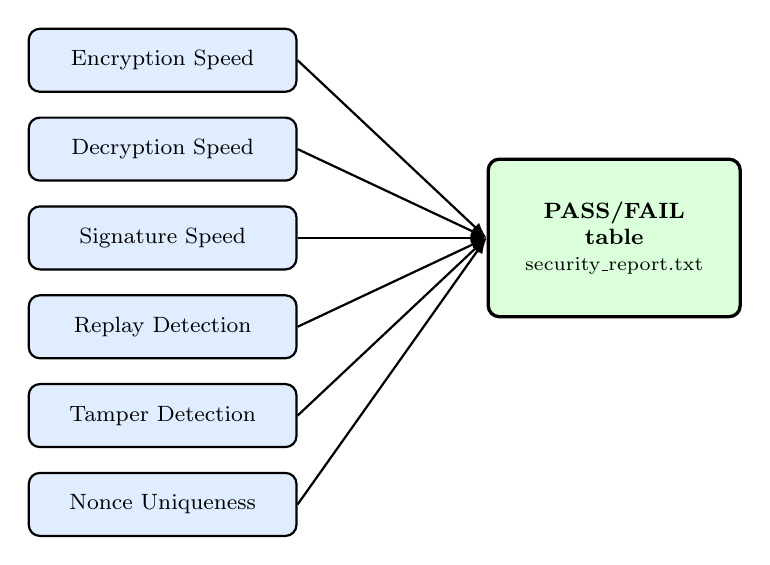
\begin{tikzpicture}[font=\footnotesize,node distance=3mm,
   t/.style={draw,thick,rounded corners,minimum width=3.4cm,minimum height=0.8cm,
             align=center,fill=boxblue}]
  \node[t] (t1) {Encryption Speed};
  \node[t,below=of t1] (t2) {Decryption Speed};
  \node[t,below=of t2] (t3) {Signature Speed};
  \node[t,below=of t3] (t4) {Replay Detection};
  \node[t,below=of t4] (t5) {Tamper Detection};
  \node[t,below=of t5] (t6) {Nonce Uniqueness};
  \node[draw,very thick,rounded corners,fill=green!14,minimum width=3.2cm,
        minimum height=2.0cm,align=center,right=24mm of t3] (rep)
       {\textbf{PASS/FAIL}\\\textbf{table}\\\scriptsize security\_report.txt};
  \foreach \n in {t1,t2,t3,t4,t5,t6}
     \draw[-{Latex[length=2mm]},thick] (\n.east) -- (rep.west);
\end{tikzpicture}
\end{center}

\subsection{Diagram 2 --- the benchmark loop}
\begin{center}
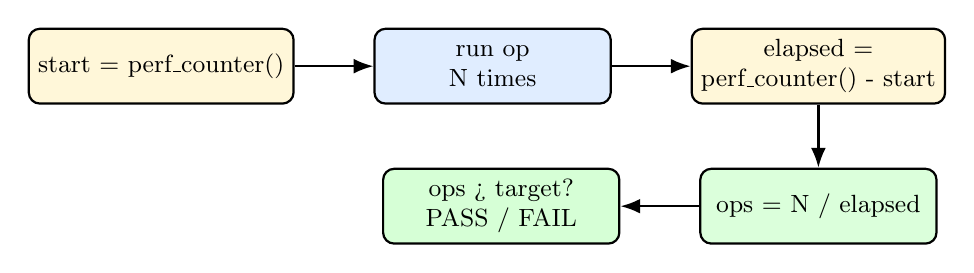
\begin{tikzpicture}[font=\small,node distance=8mm,
   s/.style={draw,thick,rounded corners,minimum width=3.0cm,minimum height=0.95cm,
             align=center}]
  \node[s,fill=boxyellow] (st) {start = perf\_counter()};
  \node[s,fill=boxblue,right=10mm of st] (lp) {run op\\N times};
  \node[s,fill=boxyellow,right=10mm of lp] (en) {elapsed =\\perf\_counter() - start};
  \node[s,fill=green!14,below=8mm of en] (ops) {ops = N / elapsed};
  \node[s,fill=green!16,left=10mm of ops] (cmp) {ops > target?\\PASS / FAIL};
  \draw[-{Latex[length=2.5mm]},thick] (st) -- (lp);
  \draw[-{Latex[length=2.5mm]},thick] (lp) -- (en);
  \draw[-{Latex[length=2.5mm]},thick] (en) -- (ops);
  \draw[-{Latex[length=2.5mm]},thick] (ops) -- (cmp);
\end{tikzpicture}
\end{center}

% =====================================================================
\section{Presentation Pack}
% =====================================================================

\subsection{Slide Outline}

\textbf{Slide 1 --- Why Measure?}
\begin{itemize}
  \item S8 proved the defences once; S9 measures them at scale.
  \item One script, \texttt{evaluate\_security.py}, six tests.
  \item Three speed tests, three correctness tests.
  \item Output: a PASS/FAIL table saved to a report file.
\end{itemize}

\textbf{Slide 2 --- The Speed Tests.}
\begin{itemize}
  \item Encryption, decryption, signing --- measured in ops/second.
  \item A high-resolution timer (\texttt{perf\_counter}) for accuracy.
  \item Targets: $>$500 ops/s for AES, $>$100 ops/s for ECDSA.
  \item Question answered: ``fast enough for real-time V2V?''
\end{itemize}

\textbf{Slide 3 --- The Detection Tests.}
\begin{itemize}
  \item Replay: re-add 100 nonces --- all 100 must be rejected.
  \item Tamper: flip one bit in 50 messages --- all 50 must fail to decrypt.
  \item Target for both: 100\%. Anything less is a fail.
  \item These quantify the S3 and S4 defences.
\end{itemize}

\textbf{Slide 4 --- Nonce Uniqueness.}
\begin{itemize}
  \item Generate 10{,}000 random 256-bit nonces.
  \item Put them in a set; count duplicates.
  \item Target: 0 collisions --- AES-GCM needs unique nonces.
  \item 256-bit values make a collision effectively impossible.
\end{itemize}

\textbf{Slide 5 --- Measuring is Not Proving.}
\begin{itemize}
  \item 6/6 PASS is strong evidence the design holds.
  \item But a test is a sample, not a mathematical proof.
  \item Honest assurance also needs review and reasoning.
  \item S9 produces a \emph{report card}, not a \emph{theorem}.
\end{itemize}

\subsection{Speaker Talking Points (about 30--60 seconds each)}

\textbf{Slide 1.} ``In the previous section we proved each defence works by
attacking it once. Section nine is the next step: instead of one attack, we
\emph{measure}. One script, evaluate\_security.py, runs six tests. Three of them
check speed --- is the cryptography fast enough? --- and three check correctness
--- do the defences catch every attack, and are the random values truly unique?
At the end it prints a clean pass-or-fail table and even saves it to a report
file, so there is a permanent record.''

\textbf{Slide 2.} ``The three speed tests run an operation in a tight loop ---
encrypting a thousand times, signing a hundred times --- and measure how long it
took with a high-resolution stopwatch called perf\_counter. Dividing the count by
the time gives operations per second. Why does this matter for security? Because
a real car sends safety messages constantly. If encryption were slow, the
security layer would make the car lag, which is itself dangerous. We set targets
in advance --- five hundred operations a second for encryption, a hundred for
signing --- and the real numbers beat them easily.''

\textbf{Slide 3.} ``The detection tests quantify the defences. The replay test
adds a hundred nonces to the cache, then tries to add every one again --- and all
one hundred repeats must be rejected. The tamper test encrypts fifty messages,
flips a single bit in each, and every one of the fifty must fail to decrypt. The
target for both is one hundred percent, and that is deliberate. Catching
ninety-nine attacks out of a hundred is not good enough when the one you miss
could be a false `I am braking' that causes a crash.''

\textbf{Slide 4.} ``The sixth test checks nonce uniqueness. Remember a nonce must
never repeat, or AES-GCM's security breaks. The test generates ten thousand
random nonces and drops them into a set, which automatically removes duplicates.
If the set still has ten thousand items, there were no collisions. And because
each nonce is 256 bits long, the chance of a clash is astronomically small ---
this is the birthday problem, but with so many possible values that a collision
is effectively impossible.''

\textbf{Slide 5.} ``One honest closing point. A result of six out of six is
genuinely strong evidence that the design holds up. But a test runs a sample of
inputs --- it is not a mathematical proof that the defence can never fail under
any input. Real-world security assurance combines testing like this with careful
code review and reasoning about the underlying cryptographic mathematics. So
think of section nine as the project's report card --- convincing evidence ---
rather than a final theorem.''

\subsection{Live-Demo Script}
\begin{enumerate}
  \item \textbf{Run it.} Execute \texttt{python tests\textbackslash
        evaluate\_security.py}.
  \item \textbf{Point at the speed rows.} ``Tens of thousands of operations a
        second --- far past the target. The cryptography is fast enough.''
  \item \textbf{Point at the detection rows.} \texttt{100/100} and \texttt{50/50}
        --- ``every single attack caught.''
  \item \textbf{Point at the summary.} \texttt{Overall: 6/6 tests PASSED}.
  \item \textbf{Show the saved report.} Open \texttt{tests\textbackslash
        security\_report.txt} --- ``a permanent, timestamped record.''
  \item \textbf{Optional break-it.} Raise the encryption threshold absurdly high
        and re-run to show a \texttt{FAIL} and \texttt{5/6}.
\end{enumerate}

\subsection{Examiner Q\&A}
\begin{enumerate}
  \item \textbf{Q: What is the purpose of \texttt{evaluate\_security.py}?}\\
        A: To measure the project --- the speed of the cryptography and the
        reliability of the defences --- and produce a pass/fail evidence report.
  \item \textbf{Q: What is throughput and why is it measured here?}\\
        A: Operations per second. It shows the cryptography is fast enough for a
        car sending safety messages in real time, so security does not cause
        dangerous lag.
  \item \textbf{Q: Why use \texttt{time.perf\_counter} rather than an ordinary clock?}\\
        A: \texttt{perf\_counter} is a high-resolution, steady stopwatch built
        for measuring short durations; a wall clock can jump and is too coarse.
  \item \textbf{Q: Why must the detection rate target be 100\%?}\\
        A: A single missed tampered or replayed safety message could cause a
        crash. For these defences, anything below 100\% is unacceptable.
  \item \textbf{Q: How does the tamper test work?}\\
        A: It encrypts 50 messages, flips one bit of ciphertext in each, and
        counts how many decryptions raise \texttt{DecryptionError}. All 50 must.
  \item \textbf{Q: What is the nonce uniqueness test checking, and why does it
        pass?}\\
        A: That 10{,}000 random nonces contain no duplicates. Because each nonce
        is 256 bits, a collision is astronomically unlikely (the birthday problem
        with a vast value space), so 0 collisions is expected.
  \item \textbf{Q: Where do the thresholds 500 and 100 come from?}\\
        A: They are project-chosen reference targets, set in advance so the
        verdict is objective. They are not formal V2V standards.
  \item \textbf{Q: Does a 6/6 pass \emph{prove} the system is secure?}\\
        A: No. It is strong \emph{evidence} from a sample of inputs, not a
        mathematical proof. Full assurance also needs code review and reasoning
        about the cryptography.
\end{enumerate}

% =====================================================================
\section{Glossary}
% =====================================================================
\begin{description}[style=nextline,leftmargin=0pt]
  \item[Security evaluation] Measuring how well a system's defences perform.
  \item[Benchmarking] Measuring code speed under controlled, repeatable conditions.
  \item[Throughput] Work done per unit time --- here operations per second (ops/s).
  \item[Operation] One run of a function being measured (one encrypt, one sign...).
  \item[time.perf\_counter] A high-resolution timer for measuring durations.
  \item[Iteration] One pass of a benchmark loop.
  \item[Threshold / target] The fixed value a measurement must beat to pass.
  \item[Pass / Fail] The verdict from comparing a measurement to its threshold.
  \item[Detection rate] Fraction of attacks a defence catches (caught / total).
  \item[Replay detection] Catching repeated nonces (tested via \texttt{ReplayCache}).
  \item[Tamper detection] Catching modified ciphertext (tested via AES-GCM).
  \item[Nonce] A value that must be used only once.
  \item[Collision] Two generated values turning out to be identical.
  \item[Nonce uniqueness] The property that generated nonces never repeat.
  \item[Birthday problem] Why collisions appear sooner than expected --- but only
        with a small value space.
  \item[set] A Python collection that automatically discards duplicates.
  \item[ReplayCache] The S4 class storing seen nonces; tested here.
  \item[DecryptionError] The exception AES-GCM raises on a tampered message.
  \item[ReplayError] The exception the ReplayCache raises on a repeated nonce.
  \item[security\_report.txt] The saved file holding the evaluation results.
  \item[Evidence vs proof] Tests give evidence; only mathematics gives proof.
\end{description}

% =====================================================================
\section{References and Further Study}
% =====================================================================
\begin{itemize}
  \item \textbf{Python time module --- \texttt{perf\_counter}} ---
        \url{https://docs.python.org/3/library/time.html#time.perf_counter}\\
        Read for: the high-resolution timer used in every speed test.
  \item \textbf{Python set type documentation} ---
        \url{https://docs.python.org/3/library/stdtypes.html#set}\\
        Read for: how the nonce-uniqueness test discards duplicates.
  \item \textbf{Benchmark (computing) (Wikipedia)} ---
        \url{https://en.wikipedia.org/wiki/Benchmark_(computing)}\\
        Read for: what benchmarking is and how to do it fairly.
  \item \textbf{Throughput (Wikipedia)} ---
        \url{https://en.wikipedia.org/wiki/Throughput}\\
        Read for: the operations-per-second idea.
  \item \textbf{Birthday problem (Wikipedia)} ---
        \url{https://en.wikipedia.org/wiki/Birthday_problem}\\
        Read for: why collisions appear sooner than intuition suggests.
  \item \textbf{Birthday attack (Wikipedia)} ---
        \url{https://en.wikipedia.org/wiki/Birthday_attack}\\
        Read for: the cryptographic version --- why nonce/hash sizes matter.
  \item \textbf{Cryptographic nonce (Wikipedia)} ---
        \url{https://en.wikipedia.org/wiki/Cryptographic_nonce}\\
        Read for: why nonce uniqueness is essential to AES-GCM.
  \item \textbf{NIST SP 800-38D --- AES-GCM} ---
        \url{https://csrc.nist.gov/pubs/sp/800/38/d/final}\\
        Read for: the official nonce rule the uniqueness test supports.
  \item \textbf{Python os.urandom documentation} ---
        \url{https://docs.python.org/3/library/os.html#os.urandom}\\
        Read for: the source of the random nonces being tested.
  \item \textbf{Software testing (Wikipedia)} ---
        \url{https://en.wikipedia.org/wiki/Software_testing}\\
        Read for: the broader idea that testing gives evidence, not proof.
\end{itemize}

\vfill
\begin{center}\footnotesize\itshape
End of Section S9 --- and of the V2V study pack (S1--S9). The evaluation report
is the project's final evidence that all six security properties hold.
\end{center}

\end{document}
